\subsection{Motivation für WiMAX}
\begin{itemize}
\item Die letzte Meile ist immer noch in der Hand von Swisscom
\item Breitbandanschlüsse sind an andere Dienste gekoppelt
\item Viele Gebiete der Erde sind an kein leitungsgebundenes NEtz angeschlossen
\item Bestehende Techniken erfüllen die Anforderungen nicht (Reichweite, Breitbandanschluss)
\end{itemize}
\subsection{Entstehung der IEEE 802.16 (WiMAX)}
\begin{itemize}
\item Globaler Standard für die Luftschnittstelle eines drahtlosen, breitbandigen Metropolitan Area Networks (MAN)
\item Übernahme der allgemeinen Prinzipien und Vorgehensweisen, die für den durchdringenden Erforlg von IEEE 802.11 Standards verantwortlich sind 
\item Reichweite im Bereich mehrere Kilometer
\item Kapazität und Durchsatz, welcher mindestens so hoch sind, wie mit drahtgebundenen Last Mile Access Technologien 
\item Breites Angebot an Diensten für Echtzeit und nciht Echtzeit Anwendungen. Entsprechend flexible Zuteilung und Garantie von QoS
\item Standard umfasst nur Layer1 und 2 des OSI Referenzmodells
\item Skalierbarkeit: Einfache Erweiterung des Netzes im Falle steigender Nachfrage
\item Ermöglichung schneller Netzinstallation (für temopräranlagen)
\item ...
\end{itemize}

Man wollte ein System erschaffen, dass sehr frei ist. Dies hat aber den Nachteil, dass die Hersteller viel Möglichkeiten zur Umsetzung haben und somit die Interoperabilität gefährdet ist. Dieses Problem wurde ähnlich wie bei Bluetooth 1.0 gelöst, nämlich mit Profilen. \\
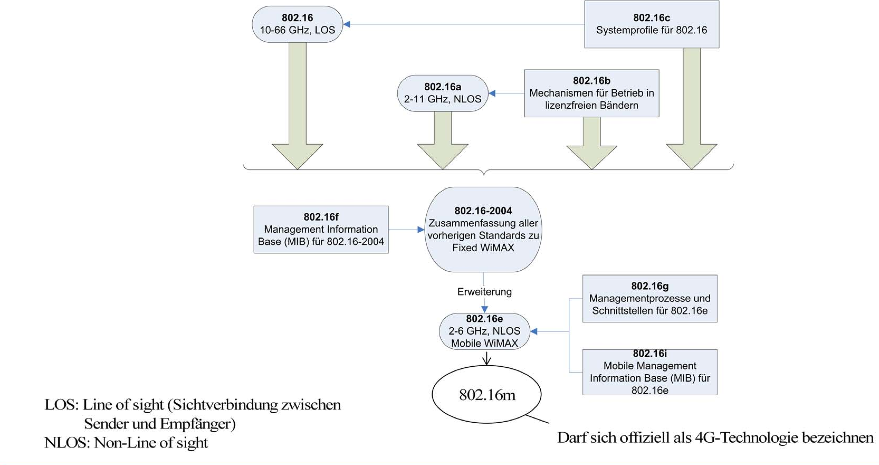
\includegraphics[width = 0.75 \linewidth]{./pics/wimax1.png} \\
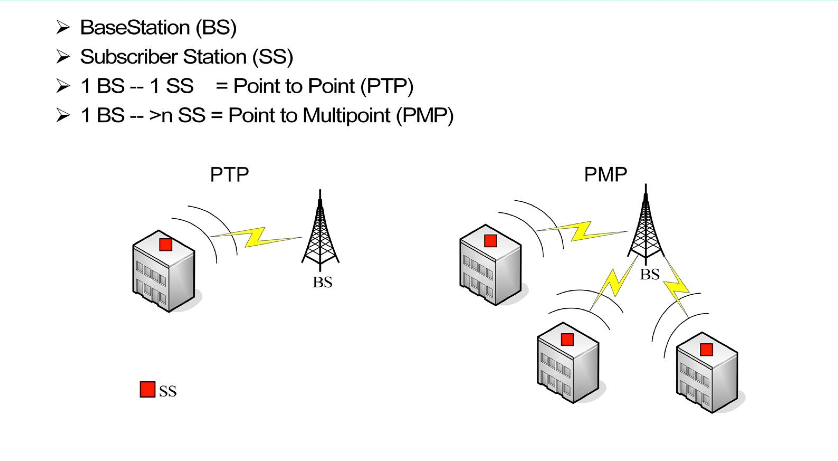
\includegraphics[width = 0.75 \linewidth]{./pics/wimax2.png} \\

\begin{itemize}
\item Verabschiedung des Standards 2001
\item Betrieb in Outdoor-Umgebung mit direkter Sichtverbindung (Line of sight: LOS) zwischen ortsfesten Sendern und Empfängern
\item Standard ist wendiger für Last Mile Access (PMP) als vielmehr für Richtfunkszenarien (PTP) geeignet
\item Trägerfrequenz 10-66 GHz
\item Max. Datenrate:134 MBit/s
\item Max. Reichweite: ca. 50 km
\end{itemize}

\begin{itemize}
\item IEEE 802.16c
\begin{itemize}
\item Jan. 2003
\item Spezifizierung von Systemprofilen
\item Definieren bestimmte MAC-, PHY- und Radio Frequency Konfigurationen (z.B. Trägerfrequenz und Kanalabstände)
\end{itemize}
\item IEEE 802.16a
\begin{itemize}
\item April 2003
\item Entwickelt für den Non Line of sight (NLOS) Einsatz
\item Erlaubt den Betrieb in lizensierten als auch in lizenzfreien Bändern
\item Trägerfrequenz 2-11 GHz
\item Max. Datenrate: ca. 70 MBit/s
\item Max. Reichweite: ca. 5 km
\end{itemize}
\item 802.16b
\begin{itemize}
\item Definiert Mechanismen und Vorkehrungen für die Koexistenz mit anderen Systemen im lizenzfreien Bereich
\item Dynamic Frequency Selection(DFS) Algorithmus
\end{itemize}
\item 802.16d
\begin{itemize}
\item Juni 2004
\item Auch unter 802.16-2004 oder "Air Interface for Fixed Bradband Wireless Access" bekannt
\item alle vorherigen Standards wurden überarbeitet und in 802.16-2004 zusammengefasst
\item Mobile SS (Subscriber Station) noch nicht unterstützt (fixed)
\end{itemize}
\item 802.16e
\begin{itemize}
\item Frühling 2006
\item Auch unter 802.16e-2005 oder mobile WiMAX bekannt
\item Geschwindigkeiten bis 125 km/h werden unterstützt
\item Mechanismen für Handover und dafür notwendige Kommunikation zwischen benachbarten BS wird definiert
\item Definiert Algorithmen zur dynamischen Sendeleistungsregelung
\item Trägerfrequenzen: 2-6 GHz
\item Datenrate: Im Bereich von mehreren 10 MBit/s (Abhängig von Kanaleigenschaften)
\end{itemize}
\item 802.16f
\begin{itemize}
\item Interoperabilität zwischen 802.16-2004 Produkten von verschiedenen Herstellern soll auf Netzwerkebene gewährleistet werden
\item Mechanismen für das Management der Komponenten und Netzte wurde definiert
\item Management Informationen Base (MIB), welche konform ist mit dem Simple Network Management Protocol Version 2 (SNMPv2)
\end{itemize}
\item 802.16g
\begin{itemize}
\item Management und Kontrollprozeduren über die Grenzen einzelner BS hinweg
\item Inter BS und auch Intersystem Kommunikation von Management- und Kontrolldaten wird spezifiziert
\end{itemize}
\item 802.16i 
\begin{itemize}
\item Definiert, basierend auf dem SNMP die Management Information Base (MIB) für das mobile Netz
\item ist als Erweiterung des 802.16f Standards für mobiles WiMAX zu sehen
\end{itemize}
\end{itemize}
\subsection{Last Mile Broadband Wireless Access (BWA)}
\includegraphics[width = 0.75 \linewidth]{./pics/wimax3.png} 
\subsection{Backhaul Anwendungen}
\includegraphics[width = 0.75 \linewidth]{./pics/wimax4.png} 

\subsection{MAC-Layer}

\begin{itemize}
\item MAC Protokoll ist verbindungsorientiert
\item Zentrales Konzept sind die Serviceflows bekannt aus LTE
\item Servicesflows definieren ein unidirektionalen Transportdienst, charakterisiert mit QoS Eigenschaften
\item SF leg fest, welcher von 5 möglichen Schedulingsdiensten im Uplink verwendet wird, um den Datenfluss zu bedinen
\begin{itemize}
\item Unsolicited Grant Service (UGS)
\item Realtime Polling Service(rtPS)
\item Non Realtime Polling Service (nrtPS)
\item Best Effort (BE)
\item Extended Realtime Variable Rate (ERT-VR) 
\end{itemize}
\item SF wird durch eine 32 Bit grosse SFID identifiziert
\item Übertragene MAC Daten sind immer einer logischen MAC Verbindung zwischen BS und SS zugeordnet
\item MAC Pakete beinhalten im Header lediglich die 16 Bit grosse Connection ID (CID), welche die logische Verbindung identifiziert
\end{itemize}

\includegraphics[width = 0.75 \linewidth]{./pics/wimaxmac.png} \\

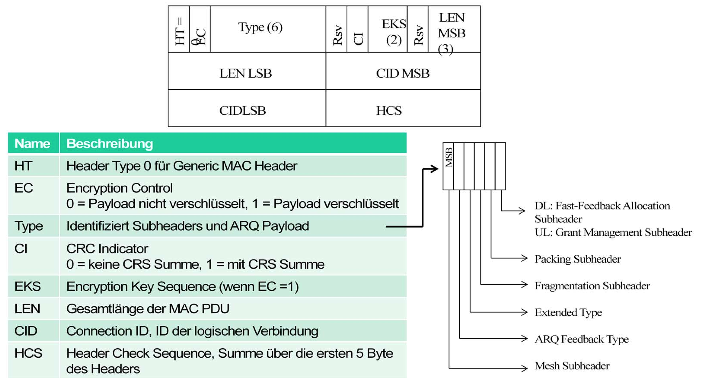
\includegraphics[width = 0.75 \linewidth]{./pics/wimaxmac2.png} \\

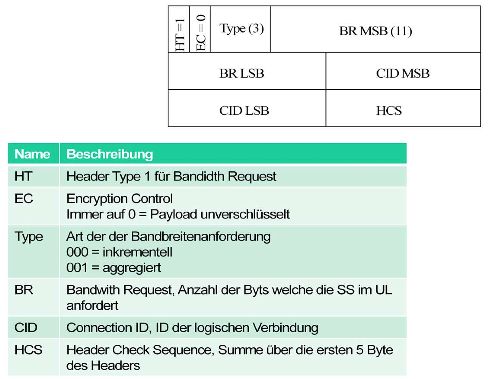
\includegraphics[width = 0.65 \linewidth]{./pics/wimaxmac3.png} \\

\subsubsection{MAC Layer: Anforderung der Bandbreite}
\begin{itemize}
\item Downlink
\begin{itemize}
\item BS ist über Datenaufkommen informiert und kann optimal reagieren, unter Berücksichtigung des QoS der einzelnen Serviceflows
\end{itemize}
\item Uplink
\begin{itemize}
\item Uplink ist über alle aktiven SS verteilt, Management der Bandbreite erschwert Lösungsansatz
\item Dynamische Bandbreitenanforderung der SS bei der BS
\item Demand Assigned Multiple Access (DAMA) Prinzip
\item Uplink Bandbreitenmanagement wird auch als Uplink Request/Grant Scheduling bezeichnet
\end{itemize}
\item Bandwidth Request
\begin{itemize}
\item PDU besteht nur aus Header
\item Inkrementell: Signalisiert den zusätzlichen Bedarf an Bandbreite
\item Aggregiert: signalisiert den gesamten Bedarf an Bandbreite
\item periodisch durch QoS Anforderungen definiert ist ein aggregierter Bandwidth Request erforderlich (selbstkorrigierend bei Verlust von Inkrementellen Bandwidth Requests)
\item Bandwidth Requests beziehen sich auf die Basic CID der SS
\item besitzt die SS mehrere Verbindungen ist sie selbst verantwortlich für die Verteilung der allozierten Bandbreite
\item Mechanismen der Bandbreitenallokation
\begin{itemize}
\item Unicast Polling
\item Multicast/Broadcast Polling
\item Piggybacked Request
\end{itemize}
\item Unicast Polling
\begin{itemize}
\item BS alloziert einer SS im Uplink Bandbreite in Form eines Unicast Request Intervalls
\item Uplink Reservation bietet nur Platz für einen Bandwidth Request von einer SS
\item SS überträgt darin den Bandwidth Request, um den aktuellen Bandbreitenbedarf zu signalisieren
\item Polling kann sowohl periodisch erfolgen als auch durch ein Poll-Me Bit angefordert werden
\end{itemize}
\item Multicast/Broadcast Polling
\begin{itemize}
\item Mehrere oder alle SS werden gepollt
\item BS reserviert im Uplink mehrere Transmission Opportunities (TO)
\item In einem Intervall können somit mehrere Bandwidth Requests gesendet werden
\item um das risiko von Kollisionen zu minimieren wird das Contention Resolution Verfahren verwendet
\item Das Intervall und die Transmission Opportunity werden mit dem Truncated Binary Exponential Backoff Verfahren zufällig gewählt
\end{itemize}
\item Piggybacked Request
\begin{itemize}
\item Bietet die Möglichkeit einen Bandwidth Request innerhalb eines Datenintervalls zu senden
\item um zu signalisieren, dass es sich um einen Piggybacked Request handelt, wird ein Subheader verwendet
\item Ein Piggybacked Request bezieht sich auf diejenigen MAC Verbindungen, über welche er geschickt wurde
\end{itemize}
\end{itemize}
\end{itemize}

\subsection{QoS - Quality of Service}
\begin{itemize}
\item ITU-T-E800 Standard: Definition von QoS
\item Mit QoS wird der Gesamteffekt der Leistungsfähigkeit eines Dienstes bezeichnet, welcher die Zufriedenheit des Dienstbenutzers bestimmt
\item QoS ist ein Konzept, um die Anforderungen eines Kommunikationsdienstes bezüglich Qualität formell spezifizieren zu können
\item QoS Parameter
\begin{itemize}
\item Throughput (Durchsatz)
\item Delay (Latenzzeit)
\item Jitter (Latenzzeit Variation)
\item Loss (Verlustrate)
\end{itemize}
\item Weitere Aspekte
\begin{itemize}
\item Verfügbarkeit des Dienstes
\item Sicherheit
\item Paketgrösse
\item Kosten
\end{itemize}
\item SLA: Service Level Agreement
\item Die eigentliche Umsetzung eines Dienstes und deren Anforderungen innerhalb eines Netzwerkes erfolgt durch spezifische Protokolle, Mechanismen und Algorithmen
\end{itemize}
\includegraphics[width = 0.75 \linewidth]{./pics/QosRef.png} \\

\begin{itemize}
\item QoS Mapping
\begin{itemize}
\item Unterschiedliche QoS Konzepte werden Aufeinander abgebildet
\item Wenn Daten von einer Protokollschicht in eine andere übergehen
\item Wenn Daten unterschiedliche Technologien passieren
\end{itemize}
\item Traffic Shaping
\begin{itemize}
\item QoS Vereinbarungen beinhalten: 
\begin{itemize}
\item Zu erbringende Leistung des Netzes
\item Charakteristik des zu erwartenden Datenverkehrs
\end{itemize}
\item Traffic Shaping sorgt dafür, dass sich der Verkehr einer Anwendung im vereinbarten Rahmen befindet
\end{itemize}
\item QoS Negotiation
\begin{itemize}
\item Methoden um erwartete Dienstgüte und Verkehrscharakteristiken zwischen verschiedenen Netzwerkinstanzen auszuhandeln
\item Offline (SLA)
\item Online (Resource Reservation Protocols)
\begin{itemize}
\item QoS Re-Negotiation (Degradierung oder Änderung der Anforderungen)
\end{itemize}
\end{itemize}
\item Admission Controll
\begin{itemize}
\item Zugangskontrolle für das Aktivieren eines neuen Dienstes
\item Check, ob Resourcen, um den Dienst zu erbringen, zum Zeitpunkt des Verbindungsaufbaus tatsächlich zur Verfügung stehen
\end{itemize}
\item QoS Monitoring
\begin{itemize}
\item Laufende oder periodische Überprüfung, ob die geforderte Dienstgüte eingehalten wird (z.B. Bufferfüllstände, aufgelaufener Delay und andere Metriken)
\item Admission Control basiert auf genauen Informationen über das Netz
\item Der Scheduling Prozess setzt QoS Anforderungen in effektive Resourcen-Allozierungen um
\item Scheduling passt sich laufen der aktuellen Situation an, um erwartete Dienstgüten zu erbringen
\end{itemize}
\item QoS Enforcement
\begin{itemize}
\item Umfasst Mechanismen, welche für die Umsetzung der QoS Vereinbarungen im System verantwortlich sind
\item Scheduling Algorithmus/Algorithmen sind typischerweise zuständig für das QoS Enforcement
\item Scheduler muss dynamisch Kompromisse zwischen sich konkurrierenden Zielen finden (Bandbreiteneffizienz, Echtzeitanforderungen, Fairness, Durchsatz usw.)
\end{itemize}
\item Resource Reservation/Association
\begin{itemize}
\item Systemressourcen werden 
\begin{itemize}
\item dynamisch durch den Scheduler den aktiven Diensten zugewiesen
\item während der Laufzeit fix reserviert (GSM, fixe Slotzuweisung)
\end{itemize}
\item In beiden Fällen werden Mechanismen benötigt, um die Resourcen beim Aktivieren des Verkehrsflussses reservieren zu können
\item Die Reservation bedeutet nicht zwingend, dass die Ressourcen während der gesamten Laufzeit nur dem einen Dienst zugewiesen sind (Bei GSM schon)
\item Temoporär ungenutzte Ressourcen können an weniger anspruchsvolle Dienste ausgeliehen werden. Die reservierten Ressourcen bleiben jedoch mit dem ursprünglichen Dienst assoziiert und können jederzeit wieder aktiviert werden
\end{itemize}
\end{itemize}

\subsubsection{QoS Mechanismen in IEEE 802.16}
\begin{itemize}
\item Service Specific Convergence Layer ist für das Mapping von Dienstklassen zuständig
\item Mit dme SF Management werden SF dem QoS entsprechend dynamisch aufgebaut, verändert und terminiert
\item Outbound and Uplink Scheduling Services gewährleisten, dass vereinbarte QoS Anforderungen eingehalten werden. Jedem SF ist ein Scheduling Service zugeordnet
\item Request Authorization prüft, ob Ressourcen vorhanden sind
\item SF Activation Model reserviert und assoziiert Ressourcen
\end{itemize}

\subsubsection{Serviceflows (SF)}
\begin{itemize}
\item Das fundamentale Konzept des QoS basiert auf SF
\item Alle Pakete werden beim Eintritt ins 802.16 Netz klassifiziert und mit einem SF assoziiert
\item SF Eigenschaften;
\begin{itemize}
\item Unidirektionaler Fluss von Paketen
\item Pakete gehören logisch zusammen
\item gemeinsame Dienstgüte benötigt
\item werden sowohl im Up- als auch im Downlink verwendet
\item ist durch sein QoSParameterSet definiert (u.a. Delay, Jitter, Datendurchsatz)
\item Besitzt 32 Bit grosse SFID
\item Besitzt Connection ID (CID), wenn SF im admitted oder active Zustand ist. Also erst, wenn eine MAC Verbindung aufgebaut wird
\end{itemize}
\item Typen von SF 
\begin{itemize}
\item provisioned SF
\item admitted SF
\item activ SF
\end{itemize}
\end{itemize}

\subsubsection{SF Type Provisioned}
\begin{itemize}
\item Wird vollumfänglich durch sein ProvisionedQoSParamSet beschriben
\item AdmittedQoSParamSet und AcitveQoSParamSet sind leer
\item Provisioned SF ist im System bekannt
\item Eine SFID ist zugewiesen
\item Keine Ressourcen reserviert oder aktiv
\item Vorkonfigurierter SF. Konfiguration wird nicht durch IEEE 802.16-2004 Standard abgedeckt
\item Besitzt keine CID
\end{itemize}

\subsubsection{SF Type Admiited und Active}
\begin{itemize}
\item Admitted
\begin{itemize}
\item Ressourcen sind reserviert
\item SFID ist zugewiesen
\item CID ist zugeteilt, MAC Verbindung wird jedoch noch nicht aktiv genutzt oder bedient
\item ist grundsätzlich ein Übergangszustand
\item besitzt AdmittedQoSParamSet
\end{itemize}
\item Active
\begin{itemize}
\item Ressourcen sind reserviert
\item SFID ist zugewiesen
\item CID ist zugeteilt
\item Datenübertragung möglich
\item Besitzt ActiveQoSParamSet, welcher den Dienst, der effektiv für den aktiven SF erbracht werden soll, definiert
\end{itemize}
\end{itemize}
\includegraphics[width = 0.75 \linewidth]{./pics/sfzustand.png} 

\subsubsection{Serviceklassen}
\begin{itemize}
\item IEEE 802.16 Standard bietet das optionale Konzept der Serviceklassen
\item Wiederkehrende Applikationen verwenden in der Regel die gleiche Servicekonfiguration (OoSParamSet)
\item Dient der Mehrfachkonfiguration von Services
\item Sind Identifikationen von QoSParamSet
\item Besitzt ASCII Namen
\item 3 Varianten um QoSParamSet zu konfigurieren:
\begin{itemize}
\item Alle QoSParameter werden explizit in der Konfiguration eines SF angegeben
\item Die Konfiguration eines SF referenziert eine Serviceklasse, von welcher die QoSParameter vollständig übernommen werden
\item Die Konfiguration einer SF referenziert eine Serviceklasse plus explizite QoSParameter. Die Konfiguration der Serviceklasse wird übernommen und punktuell durch die zusätzlichen QoSParameter ergänzt oder überschrieben
\end{itemize}
\end{itemize}

\subsubsection{Scheduling Dienste}
\begin{itemize}
\item Scheduling Dienst bestimmt grundsätzlich wie die SS mit Daten und/oder Polling Intervallen bedient wird
\item Unsolicited Grant Service (UGS)
\begin{itemize}
\item bedient höchste Anforderungen bezüglich QoS Garantien
\item bedient echtzeit Applikationen, welche periodische Daten fixer grösse generieren (z.B. VoIP ohne Silent Suppression)
\end{itemize}
\item Real Time Polling Service (rtPS)
\begin{itemize}
\item bedient echtzeit Applikationen, welche periodische Daten variabler Grösse generieren (z.B. Audio/Video Streaming Anwendungen)
\end{itemize}
\item Non Real Time Polling Service (nrtPS)
\begin{itemize}
\item bedient Applikationen, welche aperiodische Daten variabler Grösse generieren und auch toleranter sind bezüglich Delay und Jitter. (z.B. FTP mit garantierter minimaler Datenrate)
\end{itemize}
\item Best Effort Service (BE)
\begin{itemize}
\item keine Garantien betreffend Datendurchsatz, Delay und Jitter. Qualität hängt von der aktuellen Netzauslastung ab (z.B. Internetverkehr)
\end{itemize}
\item Extended Real Time Variable Rate (ERT-VR)Service
\begin{itemize}
\item Auch Extended Real Time Polling Service (ErtPS) gennant. Service ist im Standard 802.16e definiert und unterstützt Echtzeit Applikationen, wie VoIP mit Silent Suppression 
\end{itemize}
\end{itemize}

\subsection{Mobilität}
\begin{itemize}
\item Nomadischer Zugriff (802.16-2004)
\begin{itemize}
\item SS kann sich bewegen, allerdings nicht während einer laufenden Session
\end{itemize}
\item Portabler Zugriff
\begin{itemize}
\item SS kann sich während einer Session mit geringer Geschwindigkeit bewegen. Bei einem Wechsel der BS bleibt Session intakt. Während des Tellenwechsels wird die Verbindungsqualität stark eingeschränkt
\end{itemize}
\item Mobiler Zugriff (802.16e)
\begin{itemize}
\item SS wird in diesem Zusammenhang Mobile Station (MS) genannt
\item MS kann sich während einer Session mit bis zu 125 km/h bewegen, ohne die Verbindung mit BS zu verlieren
\end{itemize}
\end{itemize}

\subsubsection{Herausforderungen}
\begin{itemize}
\item Was muss zur Verfügung gestellt werden, damit Mobiler Zugriff erreicht wird und wie würde ein Ablauf eines Handovers aussehen
\item Datenbank
\item AAA (Autorisierung, Authentifizierung, Accounting)
\item Paging Area
\item Schutz der Teilnehmeridentität (verhindern von Bewegungsprofilen)
\item Messung und Auswertung der Verbindungsqualität (aktuelle und benachbarte Zelle), evtl. Handover-Entscheid
\item Anmeldung und Registration bei der neuen Zelle
\item Aufbau der Verbindung zur neuen Zelle, Abbau der Verbindung zur alten Zelle
\item Weiterleiten der evtl. zwischengespeicherten Daten
\item Update der Lokalisierungsinformation
\item ...
\end{itemize}

\subsubsection{Handover}
\begin{itemize}
\item Wechsel einer MS von der serving BS (sBS) zur target BS (tBS)
\item Gründe:
\begin{itemize}
\item Verlassen des Abdeckungsbereichs einer BS
\item Überlastsituation
\end{itemize}
\item Handover-Methoden:
\begin{itemize}
\item verbindlich
\begin{itemize}
\item Hard Handover
\end{itemize}
\item optional
\begin{itemize}
\item Macro Diversity Handover (MDHO)
\item Fast Base Station Switching (FBSS)
\end{itemize}
\end{itemize}
\item Ziel der Handover-Methoden
\begin{itemize}
\item Unterbrechungsfreier Zellenwechsel
\item Zellenwechsel soll weniger als 50 ms dauern
\end{itemize}
\end{itemize}